\graphicspath{{assessments-of-ccc/}}

\chapter{Completed Work: Assessments of Climate Change Cognition}
\label{chap:ccc}

As described above, American's are about split over acceptance of anthropogenic
climate change. Informally, Michael Ranney, then other members of our group
started questioning whether people were able to mechanistically explain how
greenhouse gases cause an increase in global mean temperature. Almost no one
could provide such an explanation. In this experiment, we sought to formally ask
whether this lack of understanding is indeed as pervasive as it seemed to be.
Critically, we suspected that a mechanistic comprehension of global climate
change might increase individual's acceptance of the reality of anthropogenic
climate change, and ultimately help pave the way towards addressing this
critical problem.

In this exploratory study, we also probed RTMD-relevant attitudes both
before and after participant's receive our explanation. In addition, we asked
participants if they experienced any surprise at our explanation. In this way,
we were able to see in what ways RTMD and multi-system learning might be
explored in future experiments.

% Ryan thinks this is unconvincing, game-show like. Could make a parallel with
% Jame's psychophysical experiments, where people could clearly know that an
% apple is read, but they need to be trained to report the basic visual
% properties of what they see preferentially over reporting "basic level"
% phenomena. The "basic pieces" of our mechanism do indeed seem new to most, but
% we have yet to formally test that part.

At present, our group has obtained responses both for 103 Berkeley
undergraduates, and 49 from two classes at UT, Brownsville. For now, we have
only prepared results from the Berkeley undergrads, and the work has been
presented in the format of a talk along with a brief mention in
\citeauthor{ranney_why_inpress}.  

\section{Overview}

The general form of the intervention was quite simple. Participants were split
into two groups. Both groups read an educational blurb regarding the mechanism
of greenhouse gasses, and indicated any surprise they may have experienced.
After this, participants completed a knowledge and attitude test. For one group,
they completed an identical knowledge and attitude test prior to the educational
blurb - making a kind of test ``sandwich'' filled with nutritious explanations
of climate change. Continuing this metaphor, the other group, with it's single
post-test is more like an ``open-faced'' (sandwich) group.\footnote{In this
    metaphor, temporal order extends from top to bottom, as with an object
    falling with gravity.}

Of central interest was verifying that almost no-one actually knows the
mechanism for climate change. And, while analyses are still in progress, we:

\begin{enumerate}
\item Assessed the effectiveness of a mechanistic explanation in eliciting
attitude shifts.
\item Assessed RTMD relationships.
\item Evaluated the predictiveness of surprise in learning and attitude shifts.
\item Observed the effects of a pre-test on participants' surprise ratings.
\end{enumerate}

In subsequent analyses, we will do a more careful analysis of the actual
learning that occurred (this has only recently been coded from written responses).


\section{Experimental Methods}

This experiment was a fairly thick observation of individuals' beliefs,
attitudes and knowledge. We sought to understand how a relatively brief 400-word
mechanistic explanation might affect these measures, as well as how this might
be modulated by prior commitment to one's own explanations.

\subsection{Participants}

As mentioned above, at present, we have collected data from 103 Berkeley
undergraduates, and 49 from two classes at the University of Texas,
Brownsville.

\subsection{Materials}

Participants received:

\begin{enumerate}
\item 400-word description of the mechanism 
by which greenhouse gases effect global mean temperature increase (in our
piloting, this description could be read in about 2 minutes)
\item RTMD attitude survey
\item 3 short essay questions testing participant knowledge of the above mechanism
\item 2 knowledge fill-in-the-blank items on light entering / exiting troposphere
\item Demographic survey
\end{enumerate}

\subsection{Procedure}

Participants were run simultaneously for each of the two classes. Instructions
were administered by the course instructor, and students received one of two
packets---placing them into one of the two groups described above. After
completing the consent form on the front of the packet, individuals proceeded to
read and answer questions. The entire experiment was completed in approximately
25 minutes.

\subsection{Analysis}

Handwritten responses were coded and placed into a spreadsheet. Given the rich
nature of these data, many analyses were employed. In brief, when appropriate,
straight t-tests were used, and in evaluating the relationships between RTMD
constructs, confirmatory factor analysis was employed.

\subsection{Results}

First off, individuals definitely did not have a clear mechanistic understanding
of how greenhouse gases contribute to global warming. Prior to instruction,
\emph{no} participants indicated anything about different kinds of radiation, or
atmospheric retention time for the sun's energy. Afterwards, though,
participants were often able to at least recall some basic details. For example,
40/103 described something about different kinds of radiation and 37/103
explained that energy was retained in the atmosphere. A more careful analysis
will be done shortly using the recently completed coding of textual items.

Participants shifted on average 14\% closer to “extreme” agreement with climate
change items. Combining groups using an imputation approach, this was
significant ($t(72)=2.28, p=.01$). There was no difference between groups on the post-test. In fact, the open-faced
group actually had a slightly greater global warming acceptance
attitude as compared to the sandwich group on average. 

Participants reported greater surprise when they were required to commit to
their own description before instruction ($t(42.1)=1.7, p=.05$). These surprise
ratings were increased from a mean of 2.3 to 3.0 on a 9-point scale. It
surprises us that their ratings are so low in general! Overall, a broad range of
surprise ratings, spanning the scale was observed. Ratings from 7 to 9 were only
observed in the Sandwich condition.

\begin{figure}[h]
\centering
\subfloat{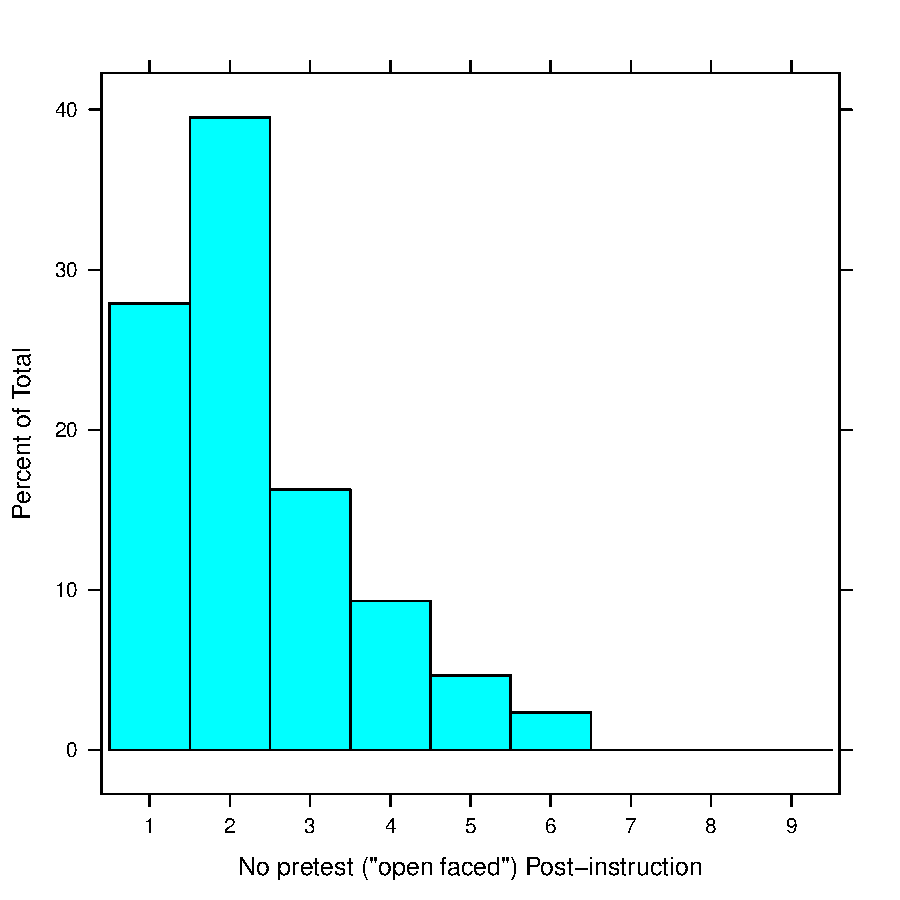
\includegraphics[width=0.5\textwidth]{hypotheses-surprisedistributions1.pdf}}
\subfloat{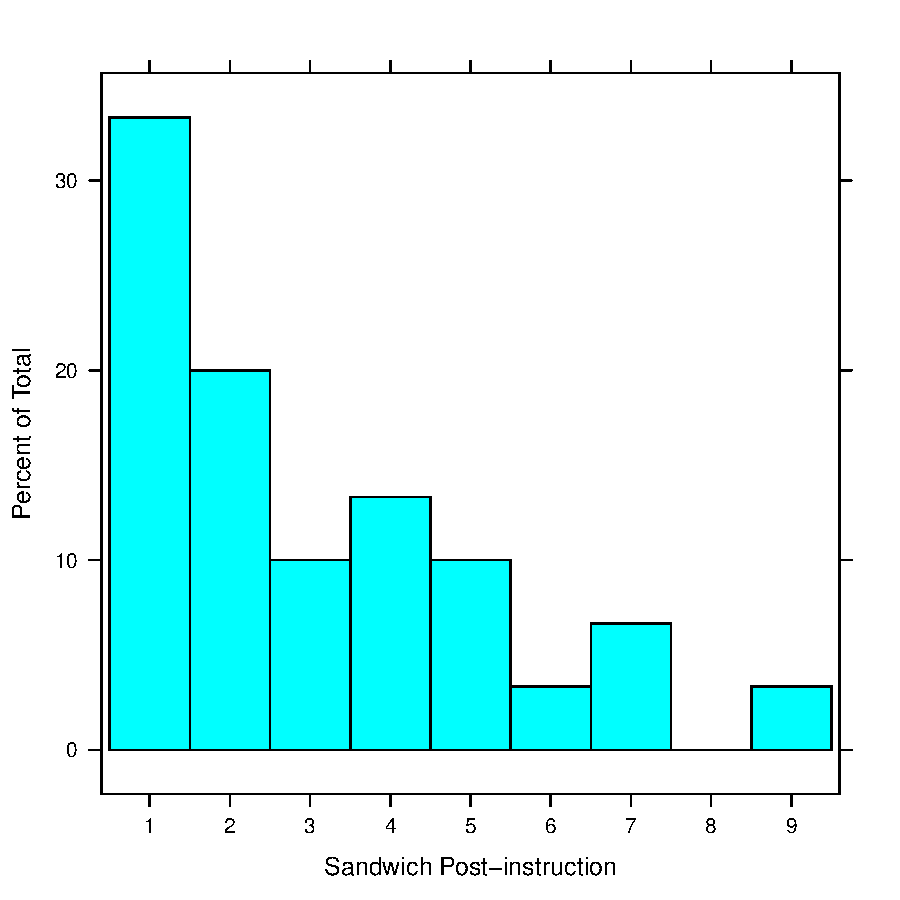
\includegraphics[width=0.5\textwidth]{hypotheses-surprisedistributions2.pdf}}
\caption{Distributions of surprise ratings for the sandwich and open-faced
groups, note the slight increase in ``1'' ratings (which may indicate resistance
to the intervention) co-occurs with an increase (from none) in ratings 7-9 in
the sandwich group.}
% For final, re-do these graphs so they have the same y-scales
\end{figure}

Note, I suspect it is unlikely that individuals experienced the same kind of
``visceral'' surprise from the blurb that can be obtained by, for example,
statistics we've used regarding things like abortion and the death penalty. And,
while it may be due to a limitation of imagination, I have difficulty imagining
an evolution item that would elicit this kind of surprise.

In addition, we replicated the relationships predicted by the RTMD theory in
another population. Confirmatory factor analysis yielded quite similar results
to simple correlation tables between the means of attitude-relevant items. In
particular, all proximal relationships held in this population (those
represented by lines in Figure~\ref{fig:rtmd}) and in each survey, either 12 or
13 out of 15 total relationships were in the direction predicted by RTMD. Less
formally, it appears that the correlations between evolution and climate change
increased after our intervention---perhaps indicating a shift in which
participants viewed climate change as part of ``real science.'' Similar
increases in anti-correlation with nationalism were observed. However, we have
not yet established appropriate statistical machinery to test the significance
of these effects.

\section{Discussion}

In general, we have established quite clearly that individuals are largely
ignorant of the mechanism via which greenhouse gases cause global warming,
suggesting that this is a reasonable object of study! More specifically, even
this (relatively dry) 400-word blurb was able to effect shifts in attitudes and
elicit non-trivial surprise ratings from individuals. It remains to see how
attitude shifts and learning are related, but the results as they are seem
sufficient basis for proceeding on an educational research program including
mechanism!


% This should be placed in the correct location above

\begin{figure}
\begin{center}
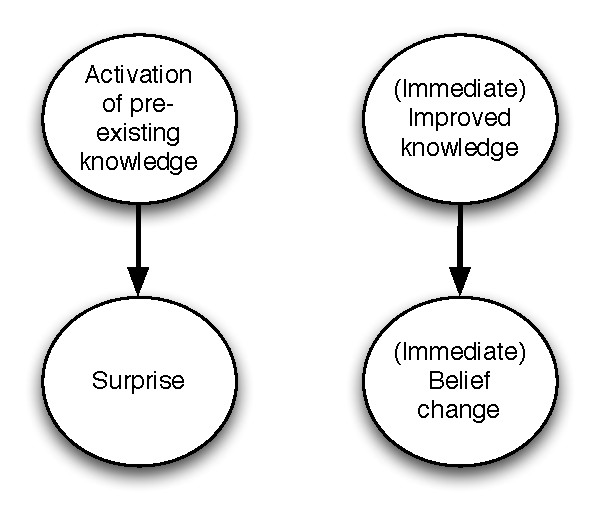
\includegraphics{causal2.pdf}
\end{center}
\caption{A graphical model representing the relationship between forms of
    psychological processing of factual information observed in
    chapter~\ref{chap:ccc}. Here, the relationship between pre-existing
    information and surprise was the result of an experimental manipulation and
    is assumed to be causal.}
\label{fig:causal-ccc}
\end{figure}
